% Main file of the group paper (IEEE Access template).
% Member 1's sections are in separate files and pulled in with \input.
% Members 2 and 3: replace the placeholder sections below with \input of your own files.
\documentclass{ieeeaccess}
\usepackage{cite}
\usepackage{amsmath,amssymb,amsfonts}
\usepackage{algorithmic}
\usepackage{graphicx}
\usepackage{textcomp}
\usepackage{array}
\usepackage{url}
\providecommand{\tbd}[1]{{\color{red}#1}}   % red = number still to be filled from the Colab run
\providecommand{\xfigwd}{0pt}                 % needed by ieeeaccess.cls when plain figure environments are used

\begin{document}
\history{Date of publication xxxx 00, 0000, date of current version xxxx 00, 0000.}
\doi{10.1109/ACCESS.2026.DOI}

\title{Bank Account Fraud Detection that Stays Fair and Stable over Time: A Time-Based Evaluation on the BAF Dataset}

\author{\uppercase{Member One}\authorrefmark{1},
\uppercase{Member Two}\authorrefmark{1}, and \uppercase{Member Three}\authorrefmark{1}}
\address[1]{Department of Computer Science, Kinnaird College for Women University, Lahore, Pakistan}

\markboth{Group XX \headeretal: Fair and Stable Bank Account Fraud Detection}
{Group XX \headeretal: Fair and Stable Bank Account Fraud Detection}

\corresp{Corresponding author: Member One (e-mail: xxx@xxx.com).}

\begin{abstract}
% Member 2 writes the abstract last (200-250 words): problem, data, method, best model with its score, main finding.
Abstract to be written after all results are in.
\end{abstract}

\begin{keywords}
Account opening fraud, concept drift, algorithmic fairness, imbalanced classification, time-based validation.
\end{keywords}

\titlepgskip=-15pt

\maketitle

% ---------------- Member 1 ----------------
% ===================== Section I: Introduction (Member 1) =====================
\section{Introduction}
\label{sec:intro}

Opening a bank account used to mean going to a branch with an identity card. Now most banks and
mobile wallets let people apply from their phone in a few minutes, and most everyday payments have
moved to digital channels. In Pakistan, the State Bank of Pakistan reports that 88\% of retail
transactions in FY2024--25 were digital, and that payments made through banking, branchless banking
and e-money wallet apps grew by 52\% to about 6.2 billion transactions in the same year
\cite{sbp2025payment}. Fraudsters use this convenience too. In account opening fraud, someone
applies with a stolen or made-up identity, gets the account approved, and then uses it to receive
illegal money or to spend the credit line that comes with it. Since the real owner of the identity
cannot be traced, the bank usually carries the loss \cite{jesus2022turning}. The problem is not a
small one: in 2024 the U.S. Federal Trade Commission received more than 1.1 million identity theft
reports, and consumers reported losing over \$12.5 billion to fraud \cite{ftc2025sentinel}.

To deal with this, banks score every new application with a machine learning (ML) model and send
the riskiest ones for rejection or manual review. Building such a model is harder than a normal
classification task, for three reasons. The first is that fraud is rare. In our data only about one
application in a hundred is fraud, so a model that never flags anyone is already 99\% accurate while
catching nothing. The second is that fraud changes over time. Fraudsters adapt to the checks they
run into, and genuine customers also change from month to month, so a model that does well on its
training months can be weaker on the months that follow \cite{dalpozzolo2018credit}. The third is
that the decision affects people. A false positive here means an honest customer is refused a bank
account, and if this happens more often to one age group than to another, the harm is not shared
equally \cite{jesus2022turning}.

A lot of the published work on fraud detection does not take these problems into account. Many
studies use public credit card data and report accuracy as their main result, even though the
classes are extremely imbalanced \cite{alarfaj2022credit, taha2020intelligent}. Others split the
data randomly and classify at the default 0.5 threshold, and a recent study on bank account opening
data did both \cite{sun2025objective}. A random split mixes later months into the training data,
which hides any drop caused by change over time. A fixed 0.5 threshold also does not match how a
bank works in practice, since it can only afford a limited number of false alarms. The Bank Account
Fraud (BAF) suite released by Jesus~\textit{et al.}~\cite{jesus2022turning} makes a more realistic
study possible. It has one million synthetic but realistic applications over eight months, a month
column for time-based evaluation, and protected attributes such as age. The original paper trained
LightGBM models on the first six months, tested them on the last two, and reported the true positive
rate at a 5\% false positive rate together with a fairness measure between age groups. It did,
however, set the 5\% threshold on the test months themselves, left a separate validation split for
the threshold as future work, and did not compare different model families under the same protocol.

In this paper we compare a majority-class baseline, a logistic regression scorecard and four ML
models from two families (random forest, LightGBM, CatBoost and a multilayer perceptron) on the BAF
Base dataset, using a strictly time-based protocol. We try to answer three research questions:
\begin{itemize}
  \item \textbf{RQ1:} Which model catches the most fraud at a fixed 5\% false positive rate?
  \item \textbf{RQ2:} How much does performance drop from the training months to the two test months?
  \item \textbf{RQ3:} Does the best model flag applicants over 50 at a different false positive rate
        from younger applicants, and what does it cost to correct this?
\end{itemize}

Our main contributions are:
\begin{enumerate}
  \item A time-based evaluation protocol for BAF without leakage. Hyperparameters are tuned on five
        forward-chaining folds over months 0--5, the 5\% FPR threshold is fixed on month 5, and
        months 6 and 7 are used only once, for the final test.
  \item A comparison of six models with the same folds, preprocessing, tuning budget and metrics,
        reported as mean $\pm$ standard deviation over the folds and month by month on the test
        period.
  \item A measurement of performance drift, including how far the false positive rate moves from
        its 5\% target when a threshold chosen on earlier data is used on later months.
  \item A fairness analysis of the false positive rate ratio between applicants over 50 and the
        rest, with the cost in recall of two corrections (group-specific thresholds and reweighing).
  \item An ablation study over six feature groups and two preprocessing steps, an error analysis of
        missed fraud cases, and a public repository that reproduces every number in the paper.
\end{enumerate}

The rest of the paper is organised as follows. Section~\ref{sec:related} reviews related work on
fraud detection, concept drift and algorithmic fairness. Section~\ref{sec:dataset} describes the
dataset, and Section~\ref{sec:method} explains the time-based validation and the rest of the
methodology. Section~\ref{sec:results} gives the results, Section~\ref{sec:fairness} the fairness
analysis and Section~\ref{sec:ablation} the ablation and error analysis.
Section~\ref{sec:discussion} discusses what we found and its limits, and
Section~\ref{sec:conclusion} concludes.
% NOTE for the group: check the \label names match the ones used in your sections.

% ============ Section II-A: Related work -- Fraud detection (Member 1) ============
% Goes inside Section II (Related Work). Member 2 writes II-B (concept drift),
% Member 3 writes II-C (algorithmic fairness); the summary table and the final
% "research gap" paragraph are joint.
\section{Related Work}
\label{sec:related}

\subsection{Fraud Detection with Machine Learning}
\label{sec:related-fraud}

\textit{Surveys.} Financial fraud detection has been reviewed many times. Al-Hashedi and
Magalingam \cite{alhashedi2021financial} reviewed data mining studies from 2009 to 2019 and grouped
them by fraud type and technique; credit card fraud was the most studied type. A later systematic
review by Ali~\textit{et al.} \cite{ali2022financial} reached the same conclusion and found support
vector machines and neural networks to be the most common models. Hilal~\textit{et al.}
\cite{hilal2022financial} focused on anomaly detection and on semi-supervised and unsupervised
methods, which are useful when labels are scarce. All three reviews point out that public data
for fraud research is limited, which is why many papers end up using the same few datasets.

\textit{Supervised models on transaction data.} Most recent supervised work uses credit card
transactions, very often the public European cardholder dataset. Alarfaj~\textit{et al.}
\cite{alarfaj2022credit} compared classical ML models with several convolutional neural networks on
that dataset and reported 99.9\% accuracy and an F1-score of 85.71\% for their best deep model.
Taha and Malebary \cite{taha2020intelligent} tuned LightGBM with Bayesian optimisation on two public
card datasets and reported 98.40\% accuracy but an F1-score of only 56.95\%, which shows how far
apart accuracy and fraud-focused metrics can be on imbalanced data. Zhao~\textit{et al.}
\cite{zhao2024improved} changed the LightGBM loss to deal with extreme imbalance and combined it with
oversampling. Gradient-boosted trees appear again and again in this line of work, which agrees with
general benchmarks showing that tree ensembles still beat deep networks on typical tabular data
\cite{grinsztajn2022tree, shwartzziv2022tabular}. The weakness shared by these studies is the evaluation:
accuracy is given as a headline metric even though fraud is rare, and none of them reports how
performance changes from one time period to the next.

\textit{Realistic evaluation and feature design.} A smaller group of papers works with data from
real fraud detection systems and tries to copy how they operate. Dal Pozzolo~\textit{et al.}
\cite{dalpozzolo2018credit} described a fraud detection system with more than 75 million
transactions over three years and showed that class imbalance, concept drift and delayed labels all
have to be handled together; they also argued that alert precision, not accuracy, is what
investigators care about. Carcillo~\textit{et al.} \cite{carcillo2021combining} added unsupervised
outlier scores as extra features for a supervised model; some scores helped, but using many of
them at once did not. Correa
Bahnsen~\textit{et al.} \cite{bahnsen2016feature} showed that aggregated features, such as how many
transactions a customer made in the last hours or days, add a lot to a fraud model. The BAF data
contains the same kind of aggregated ``velocity'' features at the application level. These papers
are close to our setting, but their data is private, so their results cannot be reproduced.

\textit{Account opening fraud and the BAF suite.} Account opening fraud is studied much less than
transaction fraud, mainly because no large public dataset existed before BAF
\cite{jesus2022turning}. BAF was generated from a real bank's application data with a tabular
generative model and extra noise for privacy, and it keeps the class imbalance, the monthly changes
and the group differences of the original data. Its authors trained 100 LightGBM configurations with
random search, trained on months 0--5 and tested on months 6--7, and reported the true positive rate
at a 5\% false positive rate and the ratio of false positive rates between age groups. Sun~\textit{et
al.} \cite{sun2025objective} compared logistic regression, an SVM, random forest, LightGBM and a GRU
on the same Base dataset. At the 0.5 threshold the classical models caught only 1--6\% of fraud,
while a class-weighted GRU caught 78\% with about 5\% precision. Their main point, that the training
objective and the operating point matter as much as the model type, supports reporting results at a
fixed false positive rate. However, they used a stratified random split instead of the month
column, tuned the classical models on a 10{,}000-row sample, and did not look at fairness.

\textit{Gap.} Taken together, the fraud detection literature either uses realistic but private
data, or public data with random splits and accuracy-style metrics. On BAF, the only public
account-opening benchmark, no study we found compares several model families under one time-based
protocol in which the 5\% FPR threshold is chosen without looking at the test months. Our study
fills this part of the gap; Sections~\ref{sec:related-drift} and \ref{sec:related-fair} cover the
drift and fairness sides.


% ---------------- Member 2 ----------------
\subsection{Concept Drift}
\label{sec:related-drift}
Member 2: related work on concept drift.

% ---------------- Member 3 ----------------
\subsection{Algorithmic Fairness}
\label{sec:related-fair}
Member 3: related work on algorithmic fairness.

% ---------------- joint ----------------
% Rows for the joint "closest studies" summary table in Section II (Member 1's share).
% Columns: Study & Data & Method & Evaluation & Reported result \\
% Members 2 and 3 add their rows (drift, fairness) so the table has 10-12 studies in total.
\begin{table*}[!t]
\centering
\caption{Summary of the closest studies (fraud detection part; drift and fairness rows to be added).}
\label{tab:related-summary}
\footnotesize
\begin{tabular}{p{2.0cm}p{3.0cm}p{3.6cm}p{3.6cm}p{3.6cm}}
\hline
\textbf{Study} & \textbf{Data} & \textbf{Method} & \textbf{Evaluation} & \textbf{Reported result} \\
\hline
Jesus \textit{et al.} 2022 \cite{jesus2022turning} & BAF suite (Base + 5 variants), 1M rows each & LightGBM, 100 random-search configs & Train months 0--5, test 6--7; TPR at 5\% FPR; FPR ratio by age & Benchmark of performance and fairness across variants \\
Sun \textit{et al.} 2025 \cite{sun2025objective} & BAF Base & LR, SVM, RF, LightGBM, class-weighted GRU & Stratified random 80/20 split; 0.5 threshold & GRU: 78\% fraud recall, $\sim$5\% precision, AUC 0.88 \\
Dal Pozzolo \textit{et al.} 2018 \cite{dalpozzolo2018credit} & 75M+ real card transactions (private), 3 years & Separate models for feedback and delayed labels, aggregated & Realistic alert-feedback setting; alert precision & Learning strategy handles imbalance, drift and verification latency \\
Carcillo \textit{et al.} 2021 \cite{carcillo2021combining} & Real card transactions (private) & Unsupervised outlier scores added to supervised model & Real annotated data & Some outlier scores help; using many at once does not \\
Taha \& Malebary 2020 \cite{taha2020intelligent} & Two public card datasets & LightGBM with Bayesian tuning & Accuracy, AUC, precision, F1 & Acc. 98.40\%, AUC 92.88\%, F1 56.95\% \\
Alarfaj \textit{et al.} 2022 \cite{alarfaj2022credit} & European cardholder dataset & ML models vs. CNNs & Accuracy, precision, F1, AUC & Acc. 99.9\%, F1 85.71\%, AUC 98\% \\
\hline
\end{tabular}
\end{table*}

% Joint: final "research gap" paragraph for Section II.

% ---------------- Member 1 ----------------
% ===================== Section III: Dataset (Member 1) =====================
\section{Dataset}
\label{sec:dataset}

\subsection{Source and Licence}

We use the Base dataset of the Bank Account Fraud (BAF) suite \cite{jesus2022turning}, which is
available on Kaggle and GitHub \cite{baf2022kaggle} under the CC BY-NC-ND 4.0 licence, so it may be
used for non-commercial research without changes to the data itself. The suite was created by Feedzai
from a real, anonymised dataset of online bank account applications at a large consumer bank. Each
row is a synthetic application produced by a CTGAN generative model, and noise was added to give a
degree of differential privacy, so no row belongs to a real person \cite{jesus2022turning}. The
fraud labels in the original data were collected several months after the accounts were opened.
The suite contains six datasets of one million rows each; the Base dataset keeps the natural biases
of the original data, while the five variants add controlled types of bias. We use only the Base
dataset, as required by the topic.

\subsection{Size and Features}

The Base dataset has \tbd{1,000,000} applications and \tbd{32} columns: the label
\texttt{fraud\_bool}, the application \texttt{month} (0 to 7), and 30 features. Five features are
categorical with anonymised levels (\texttt{payment\_type}, \texttt{employment\_status},
\texttt{housing\_status}, \texttt{source}, \texttt{device\_os}); the rest are numeric or binary.
The data contains three attributes that are treated as protected in the BAF paper: age
(\texttt{customer\_age}, rounded to the decade), income (\texttt{income}, in deciles) and
employment status. For the description and for the ablation study we group the features into six
groups by what they describe (Table~\ref{tab:groups}). The application velocity group holds
aggregated counts, such as the number of applications per hour in the last 6 hours, 24 hours and 4
weeks, or the number of applications from the same zip code in the last 4 weeks.

\begin{table}[!t]
\centering
\caption{Feature groups used in the dataset description and the ablation study.}
\label{tab:groups}
\footnotesize
\setlength{\tabcolsep}{3.5pt}
\begin{tabular}{>{\raggedright\arraybackslash}p{1.55cm}>{\raggedright\arraybackslash}p{6.3cm}}
\hline
Group & Features \\
\hline
Applicant (4) & \texttt{\footnotesize income}, \texttt{\footnotesize customer\_\allowbreak age}, \texttt{\footnotesize employment\_\allowbreak status}, \texttt{\footnotesize housing\_\allowbreak status} \\
Address history (2) & \texttt{\footnotesize prev\_\allowbreak address\_\allowbreak months\_\allowbreak count}, \texttt{\footnotesize current\_\allowbreak address\_\allowbreak months\_\allowbreak count} \\
Email and phone (4) & \texttt{\footnotesize name\_\allowbreak email\_\allowbreak similarity}, \texttt{\footnotesize email\_\allowbreak is\_\allowbreak free}, \texttt{\footnotesize phone\_\allowbreak home\_\allowbreak valid}, \texttt{\footnotesize phone\_\allowbreak mobile\_\allowbreak valid} \\
Application velocity (7) & \texttt{\footnotesize velocity\_\allowbreak 6h}, \texttt{\footnotesize velocity\_\allowbreak 24h}, \texttt{\footnotesize velocity\_\allowbreak 4w}, \texttt{\footnotesize zip\_\allowbreak count\_\allowbreak 4w}, \texttt{\footnotesize bank\_\allowbreak branch\_\allowbreak count\_\allowbreak 8w}, \texttt{\footnotesize date\_\allowbreak of\_\allowbreak birth\_\allowbreak distinct\_\allowbreak emails\_\allowbreak 4w}, \texttt{\footnotesize days\_\allowbreak since\_\allowbreak request} \\
Credit and banking (6) & \texttt{\footnotesize credit\_\allowbreak risk\_\allowbreak score}, \texttt{\footnotesize proposed\_\allowbreak credit\_\allowbreak limit}, \texttt{\footnotesize intended\_\allowbreak balcon\_\allowbreak amount}, \texttt{\footnotesize payment\_\allowbreak type}, \texttt{\footnotesize bank\_\allowbreak months\_\allowbreak count}, \texttt{\footnotesize has\_\allowbreak other\_\allowbreak cards} \\
Device and session (6) & \texttt{\footnotesize device\_\allowbreak os}, \texttt{\footnotesize source}, \texttt{\footnotesize session\_\allowbreak length\_\allowbreak in\_\allowbreak minutes}, \texttt{\footnotesize keep\_\allowbreak alive\_\allowbreak session}, \texttt{\footnotesize device\_\allowbreak distinct\_\allowbreak emails\_\allowbreak 8w}, \texttt{\footnotesize foreign\_\allowbreak request} \\
\hline
\end{tabular}
\end{table}


\subsection{Class Balance and Time}

Only \tbd{11,029} applications (\tbd{1.10\%}) are fraudulent. Fig.~\ref{fig:months} shows the
number of applications and the fraud rate in each month. \tbd{Describe: months differ in size from
X to Y applications; fraud rate ranges from A\% (month M) to B\% (month N); the test months have a
higher/lower rate than the development months.} This means that the prior probability of fraud
itself moves over time, which is one of the reasons why a threshold chosen on earlier months may
not give the same false positive rate later.

\begin{figure}[!t]
\centering
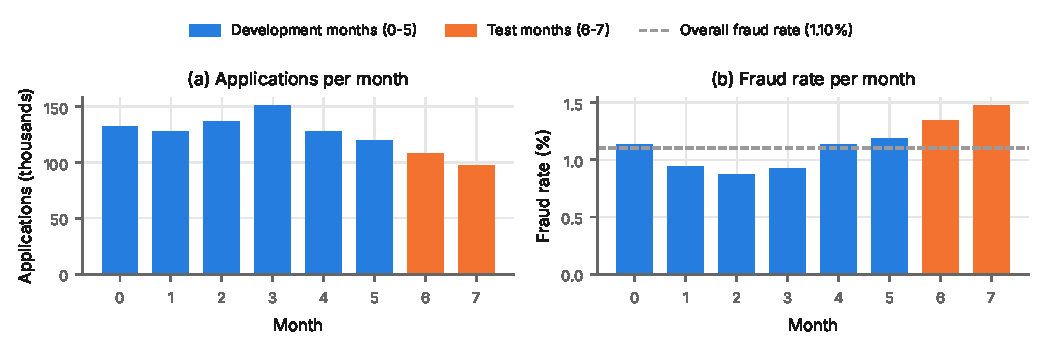
\includegraphics[width=\columnwidth]{figures/eda_months.pdf}
\caption{Applications (a) and fraud rate (b) per month in the BAF Base dataset. Months 0--5 (blue)
are used for development and months 6--7 (orange) for testing; the dashed line is the overall fraud
rate.}
\label{fig:months}
\end{figure}

\subsection{Protected Attribute: Age}

Fig.~\ref{fig:age} shows the age distribution and the fraud rate per age decade. \tbd{X\%} of
applicants are in the group older than 50 used in our fairness analysis. Their fraud rate is
\tbd{A\%}, against \tbd{B\%} for applicants aged 50 or under. \tbd{Comment on the trend of fraud
rate with age.} Because the older group has a higher base rate of fraud, a model can learn to rely
on age, which would raise the false positive rate for genuine older applicants. This is what RQ3
measures.

\begin{figure}[!t]
\centering
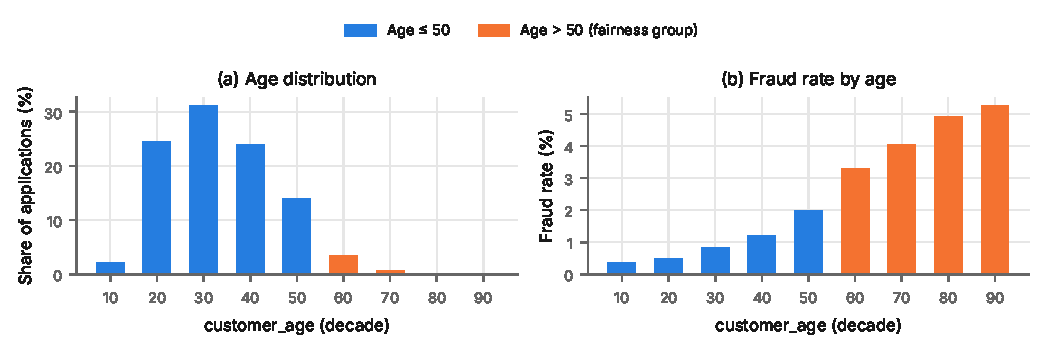
\includegraphics[width=\columnwidth]{figures/eda_age.pdf}
\caption{Share of applications (a) and fraud rate (b) by \texttt{customer\_age} decade. Orange bars
are the group older than 50 used in the fairness analysis.}
\label{fig:age}
\end{figure}

\subsection{Missing Values}

The file has no empty cells, but the datasheet states that in five features a value of $-1$ means
``missing'' and that any negative value of \texttt{intended\_balcon\_amount} is missing
\cite{baf2022kaggle}. After decoding them, \tbd{describe rates: e.g. intended\_balcon\_amount X\%,
prev\_address\_months\_count Y\%, \ldots, session\_length\_in\_minutes Z\%}
(Fig.~\ref{fig:missing}a). Missingness is not random: \tbd{describe which missing values go with
higher/lower fraud rates} (Fig.~\ref{fig:missing}b). For this reason we add a binary
``was missing'' indicator for every such feature instead of only filling the gap.

\begin{figure}[!t]
\centering
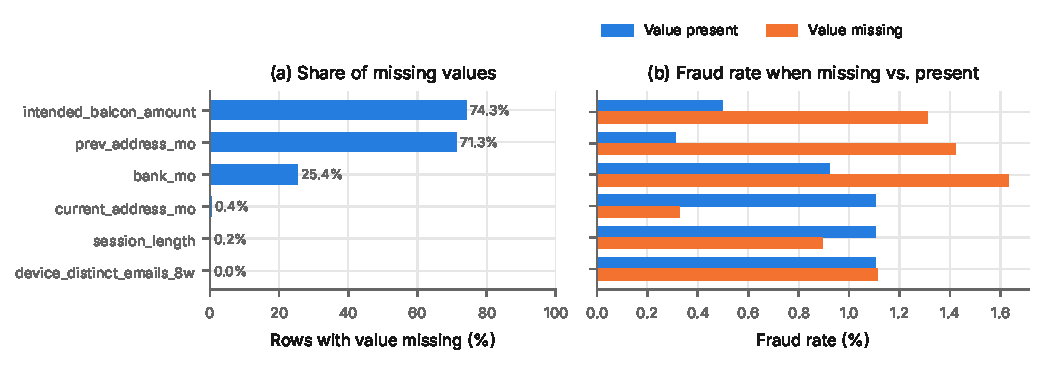
\includegraphics[width=\columnwidth]{figures/eda_missing.pdf}
\caption{(a) Share of applications where each feature is missing after decoding the datasheet's
missing-value codes. (b) Fraud rate when the value is present (blue) and missing (orange).}
\label{fig:missing}
\end{figure}

\subsection{Cleaning and Preprocessing}

We made the following cleaning decisions, all of which are applied before any split and none of
which use the label:
\begin{itemize}
  \item the coded missing values described above are converted to real missing values;
  \item \texttt{device\_fraud\_count} \tbd{takes only the value 0} in the Base file, so it carries
        no information and is removed;
  \item \texttt{month} is used only to define the time-based split and never as a model input,
        because the test months 6 and 7 are values the model would never have seen in training;
  \item \texttt{velocity\_6h} has \tbd{N} negative values; they lie inside the range documented in the
        datasheet and are not described as missing, so we keep them as they are, and negative
        \texttt{credit\_risk\_score} values are valid scores;
  \item \tbd{there are no duplicate rows}, and the categorical features are kept as strings for
        one-hot encoding.
\end{itemize}
This leaves 29 input features. All steps that learn from the data, such as imputation, encoding and
scaling, are fitted later inside each training fold (Section~\ref{sec:method-prep}).

% ============ Section IV: Validation and Methodology (Member 1) ============
% Topic 9 asks for "Validation: time-based split by month" as Section 4; the brief's general
% section list asks for the methodology content (pipeline, models, tuning, metrics, versions).
% Both are covered here.
\section{Validation and Methodology}
\label{sec:method}

Fig.~\ref{fig:pipeline} gives an overview of the whole pipeline. One rule is behind every choice in
this section: no information from a later month, and nothing from the test months, may reach a model
or a decision before that model is evaluated.

\begin{figure*}[!t]
\centering
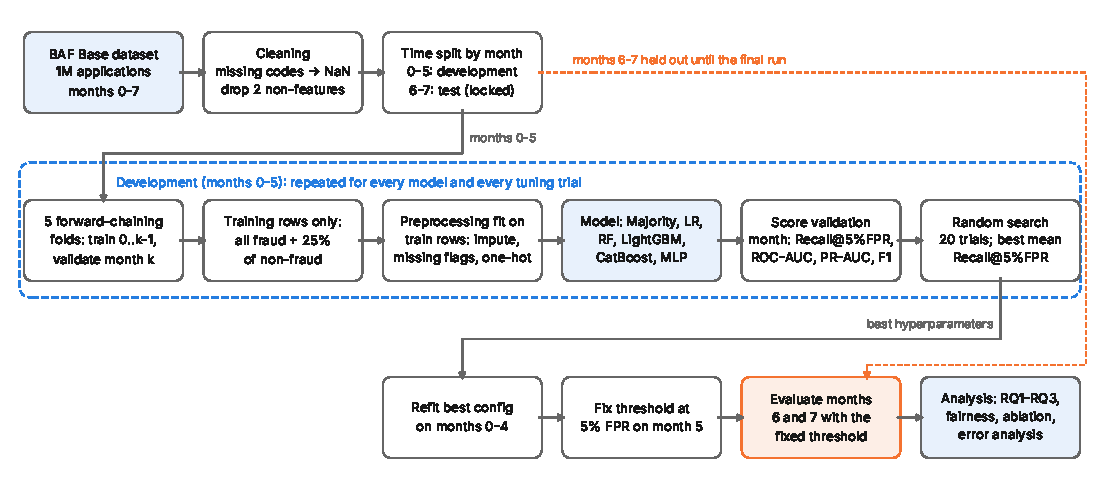
\includegraphics[width=\textwidth]{figures/pipeline.pdf}
\caption{Experimental pipeline. Months 0--5 are used for model selection with five forward-chaining
folds, and all sampling and preprocessing is fitted on the training rows of each fold only. The best
configuration of each model is refitted on months 0--4, its decision threshold is fixed at a 5\%
false positive rate on month 5, and it is then evaluated once on months 6 and 7.}
\label{fig:pipeline}
\end{figure*}

\subsection{Time-Based Split by Month}
\label{sec:method-split}

We follow the split of the original BAF paper \cite{jesus2022turning}. Months 0--5 are used for
development, and months 6 and 7 are kept as the test period. The months are never shuffled. Inside
the development period we use forward-chaining (expanding window) cross-validation
\cite{cerqueira2020evaluating}. Fold $k$ ($k=1,\dots,5$) trains on months $0$ to $k-1$ and validates
on month $k$, so each validation month comes strictly after the data the model was trained on.
Table~\ref{tab:folds} gives the size and fraud rate of each fold. With five folds we can report the
mean and standard deviation of every metric and still respect the order of time, which a shuffled
$k$-fold split would not do \cite{kaufman2012leakage}. The downside is that early folds train on less
data than later ones, so the variation between folds comes from both training size and drift. We
keep this in mind when we read the standard deviations.

\begin{table}[!t]
\centering
\caption{Forward-chaining folds on the development months (training sizes before sampling).}
\label{tab:folds}
\footnotesize
\setlength{\tabcolsep}{3.5pt}
\begin{tabular}{ccrrrr}
\hline
Fold & Train mon. & Train rows & Fraud & Val. mon. & Fraud \\
\hline
1 & 0 & 132,440 & 1.13\% & 1 & 0.94\% \\
2 & 0--1 & 260,060 & 1.04\% & 2 & 0.87\% \\
3 & 0--2 & 397,039 & 0.98\% & 3 & 0.92\% \\
4 & 0--3 & 547,975 & 0.97\% & 4 & 1.14\% \\
5 & 0--4 & 675,666 & 1.00\% & 5 & 1.18\% \\
\hline
\end{tabular}
\end{table}


After model selection, each model is refitted with its best hyperparameters on months 0--4. Month 5
is only used to fix the decision threshold (and, for the boosting models and the MLP, for early
stopping), and then months 6 and 7 are scored once. We chose this instead of refitting on all of
months 0--5, because setting the threshold on the test months would mean tuning on test data. The
original BAF study set its threshold on the test period and mentioned a separate validation split as
future work \cite{jesus2022turning}. Since our threshold comes from an earlier month, the false
positive rate on months 6 and 7 will not be exactly 5\%. We report the value that is actually
reached, because the gap is itself a sign of drift (RQ2).

\subsection{Preprocessing}
\label{sec:method-prep}

The cleaning steps in Section~\ref{sec:dataset} (decoding the missing values and removing
\texttt{month} and \texttt{device\_fraud\_count}) do not learn anything from the data, so they are
applied to the whole file once. Every step that does learn from the data is part of a scikit-learn
pipeline \cite{pedregosa2011scikit} and is fitted inside each fold on the training rows only:
{\sloppy
\begin{itemize}
  \item numeric features: missing values are replaced by the training median, and a 0/1 indicator
        column is added for each feature that had missing values, since missingness itself is
        related to fraud (Section~\ref{sec:dataset});
  \item categorical features (\texttt{payment\_type}, \texttt{employment\_status},
        \texttt{housing\_status}, \texttt{source}, \texttt{device\_os}): one-hot encoding, where
        categories not seen in training are ignored at prediction time;
  \item standardisation to zero mean and unit variance for logistic regression and the MLP, which are
        sensitive to feature scale. The tree models use the unscaled values.
\end{itemize}
}

\subsection{Handling Class Imbalance}
\label{sec:method-imbalance}

Fraud is only about 1\% of applications. We use two simple measures that are common in the
imbalanced learning literature \cite{johnson2019survey}. First, models that support it are trained
with balanced class weights, so mistakes on the fraud class count more. Second, during training we
keep every fraud application but only a random 25\% of the legitimate ones. This cuts each training
set to about a quarter of its size, which is what made a 20-trial search over five folds possible for
every model on our hardware. The sampling is only applied to training rows. Validation and test
months are always scored in full and at their real fraud rate. Our main metric takes its threshold
from the scores of the legitimate applications in the month being evaluated, so under-sampling the
training data does not change how it is measured. Removing the class weights is one of the ablation
settings (Section~\ref{sec:ablation}).

\subsection{Models}
\label{sec:method-models}

We compare two baselines and four ML models from two families (tree-based and neural):
\begin{itemize}
  \item \textbf{Majority class.} Always predicts ``not fraud''. Every application gets the same
        score, so it shows what accuracy looks like when no fraud is caught.
  \item \textbf{Logistic regression scorecard.} A linear model with L2 regularisation and balanced
        class weights. It is the traditional choice in credit risk because each coefficient can be
        read directly, so it shows how much the non-linear models add.
  \item \textbf{Random forest} \cite{breiman2001random}. An ensemble of decision trees trained on
        bootstrap samples with random feature subsets. It handles mixed feature types and
        interactions with little tuning, and it is a common strong baseline for tabular data.
  \item \textbf{LightGBM} \cite{ke2017lightgbm}. Gradient-boosted trees with histogram-based
        splits. It is the model used in the original BAF benchmark \cite{jesus2022turning}.
  \item \textbf{CatBoost} \cite{prokhorenkova2018catboost}. Gradient-boosted trees with ordered
        boosting and native handling of categorical features.
  \item \textbf{Multilayer perceptron (MLP).} A feed-forward neural network on the scaled, one-hot
        encoded features. It represents the neural family. Tree ensembles are expected to do better
        on tabular data \cite{grinsztajn2022tree, shwartzziv2022tabular}, and including an MLP lets
        us check this on BAF.
\end{itemize}
% Members 2 and 3: add one sentence each on your final LightGBM / CatBoost / MLP settings
% (e.g. early stopping rounds, MLP layers and optimiser).

\subsection{Hyperparameter Tuning}
\label{sec:method-tuning}

Every model gets the same budget: a random search \cite{bergstra2012random} over 20 configurations,
each evaluated on all five folds. The score of a configuration is its mean recall at 5\% FPR over the
five validation months, and the configuration with the highest mean is chosen. The test months play
no part in this. Table~\ref{tab:tuning} lists the search ranges and the chosen values. The majority
baseline has no hyperparameters.

\begin{table}[!t]
\centering
\caption{Random-search ranges (20 trials per model) and selected values.}
\label{tab:tuning}
\footnotesize
\setlength{\tabcolsep}{3.5pt}
\begin{tabular}{llll}
\hline
Model & Hyperparameter & Search range & Selected \\
\hline
Log. reg. & C & log-unif. $[10^{-3}, 10^{2}]$ & 0.00826 \\
\hline
Rand. forest & n\_estimators & integer $[100, 300]$ & 233 \\
 & max\_depth & \{8, 12, 16, 20, 24\} & 20 \\
 & min\_samples\_leaf & \{1, 5, 10, 25, 50, 100\} & 5 \\
 & max\_features & \{sqrt, 0.2, 0.33\} & 0.2 \\
 & max\_samples & uniform $[0.05, 0.30]$ & 0.216 \\
\hline
LightGBM & learning\_rate & log-unif. $[0.02, 0.3]$ & 0.0227 \\
 & num\_leaves & integer $[15, 255]$ & 35 \\
 & max\_depth & \{-1, 6, 8, 12\} & 8 \\
 & min\_child\_samples & integer $[20, 199]$ & 154 \\
 & subsample & uniform $[0.6, 1.0]$ & 0.605 \\
 & colsample\_bytree & uniform $[0.5, 1.0]$ & 0.796 \\
 & reg\_lambda & log-unif. $[10^{-3}, 10]$ & 0.0634 \\
\hline
CatBoost & learning\_rate & log-unif. $[0.05, 0.3]$ & 0.0756 \\
 & depth & \{4, 6, 8, 10\} & 4 \\
 & l2\_leaf\_reg & log-unif. $[1, 30]$ & 1.06 \\
 & bagging\_temperature & uniform $[0, 1]$ & 0.808 \\
\hline
\end{tabular}
\end{table}


\subsection{Evaluation Metrics}
\label{sec:method-metrics}

Let $s(x)$ be the score a model gives to application $x$ and $t$ a threshold, where $x$ is flagged as
fraud when $s(x) > t$. Following \cite{jesus2022turning}, our main metric is the recall (true
positive rate) at a 5\% false positive rate:
\begin{align}
  t_{5\%} &= \min\{\,t : \mathrm{FPR}(t) \le 0.05\,\}, \\
  \mathrm{Recall@5\%FPR} &= \mathrm{TPR}(t_{5\%}),
\end{align}
where $\mathrm{FPR}(t)$ is the share of legitimate applications with $s(x)>t$ and
$\mathrm{TPR}(t)$ is the share of fraudulent ones. It answers a practical question: how much fraud is
caught if the bank accepts that 5\% of genuine customers are wrongly flagged? In the validation
folds, $t_{5\%}$ is computed on the validation month itself, so the metric measures how well a model
ranks applications. On the test months, $t_{5\%}$ is the threshold fixed on month 5.

We also report ROC-AUC, PR-AUC (average precision), which says more than ROC-AUC when the positive
class is rare \cite{saito2015precision}, and the F1-score at the same threshold. Accuracy is only
reported for the majority baseline, to show why we do not use it. For the fairness analysis
(Section~\ref{sec:fairness}) we use the false positive rate ratio between applicants over 50 and
those aged 50 or under, defined as the lower group FPR divided by the higher one, so that 1 means
equal treatment \cite{jesus2022turning}. We only call one model better than another when its lead in
mean recall at 5\% FPR is larger than the standard deviation across folds. The fold-by-fold scores
are shown as box plots in Section~\ref{sec:results}.

\subsection{Hardware and Software}
\label{sec:method-env}

The baselines and the random forest were run on the free Google Colab CPU runtime (2 virtual cores
of an Intel Xeon CPU at 2.20\,GHz, 12.7\,GB of RAM) with Python 3.13, scikit-learn 1.6.1, pandas
2.2.3, NumPy 2.4.6 and SciPy 1.16.3. We use a fixed random seed (42) for sampling, model training and
the random search. The versions are saved by \texttt{scripts/00\_environment.py} and listed in the
repository.
% Members 2 and 3: add your LightGBM / CatBoost / PyTorch versions and machine if different.


% ---------------- Member 2 ----------------
\section{Results}
\label{sec:results}
Member 2: main results table (mean $\pm$ std), box plot, recall at 5\% FPR per model and per month,
ROC/PR curves, confusion matrix, learning curves, feature importance.
\begin{table*}[!t]
\centering
\caption{Baselines and random forest: mean $\pm$ std over the five validation folds, and the test months with the threshold fixed on month 5. (To be merged into the main results table.)}
\label{tab:member1-results}
\footnotesize
\begin{tabular}{lcccc|ccc}
\hline
 & \multicolumn{4}{c|}{Validation folds (months 1--5)} & \multicolumn{3}{c}{Test} \\
Model & Recall@5\%FPR & ROC-AUC & PR-AUC & F1 & Recall M6 & Recall M7 & FPR M6--7 \\
\hline
Majority class & 0.000 $\pm$ 0.000 & 0.500 $\pm$ 0.000 & 0.010 $\pm$ 0.001 & 0.000 $\pm$ 0.000 & 0.000 & 0.000 & 0.00\% \\
Logistic regression & 0.516 $\pm$ 0.020 & 0.887 $\pm$ 0.014 & 0.134 $\pm$ 0.018 & 0.161 $\pm$ 0.018 & 0.522 & 0.441 & 4.56\% \\
Random forest & 0.503 $\pm$ 0.022 & 0.881 $\pm$ 0.018 & 0.125 $\pm$ 0.018 & 0.157 $\pm$ 0.020 & 0.521 & 0.496 & 4.81\% \\
\hline
\end{tabular}
\end{table*}


% ---------------- Member 3 ----------------
\section{Fairness Analysis}
\label{sec:fairness}
Member 3: false positive rate ratio between age groups and the cost of the two corrections.

\section{Ablation and Error Analysis}
\label{sec:ablation}
Member 3: ablation over feature groups and preprocessing steps; missed fraud cases.

\section{Discussion}
\label{sec:discussion}
Member 3: answers to RQ1--RQ3, comparison with published results, practical meaning, threats to validity.

% ---------------- Member 2 ----------------
\section{Conclusion and Future Work}
\label{sec:conclusion}
Member 2: findings and two or three next steps.

% ---------------- joint ----------------
\section*{Declarations}
\textit{Author contributions (CRediT):} to be added.\\
\textit{Data and code availability:} The BAF dataset is available from Kaggle under the CC BY-NC-ND 4.0
licence. Our code is available at \url{https://github.com/XXXX}.\\
\textit{Conflict of interest:} The authors declare no conflict of interest.

\bibliographystyle{IEEEtran}
\bibliography{references_member1}

\EOD
\end{document}
